\documentclass{article}

\usepackage{graphicx}
\usepackage{tikz}
\usepackage{tikzsymbols}
\usetikzlibrary{calc,patterns,shapes.geometric}
\pagestyle{empty}
\usepackage[margin=0pt]{geometry}
\geometry{papersize={14in,12in}}

\def\centerarc[#1](#2)(#3:#4:#5){\draw[#1] ($(#2)+({#5*cos(#3)},{#5*sin(#3)})$) arc (#3:#4:#5);}

\begin{document}
	\begin{figure}
		\centering
		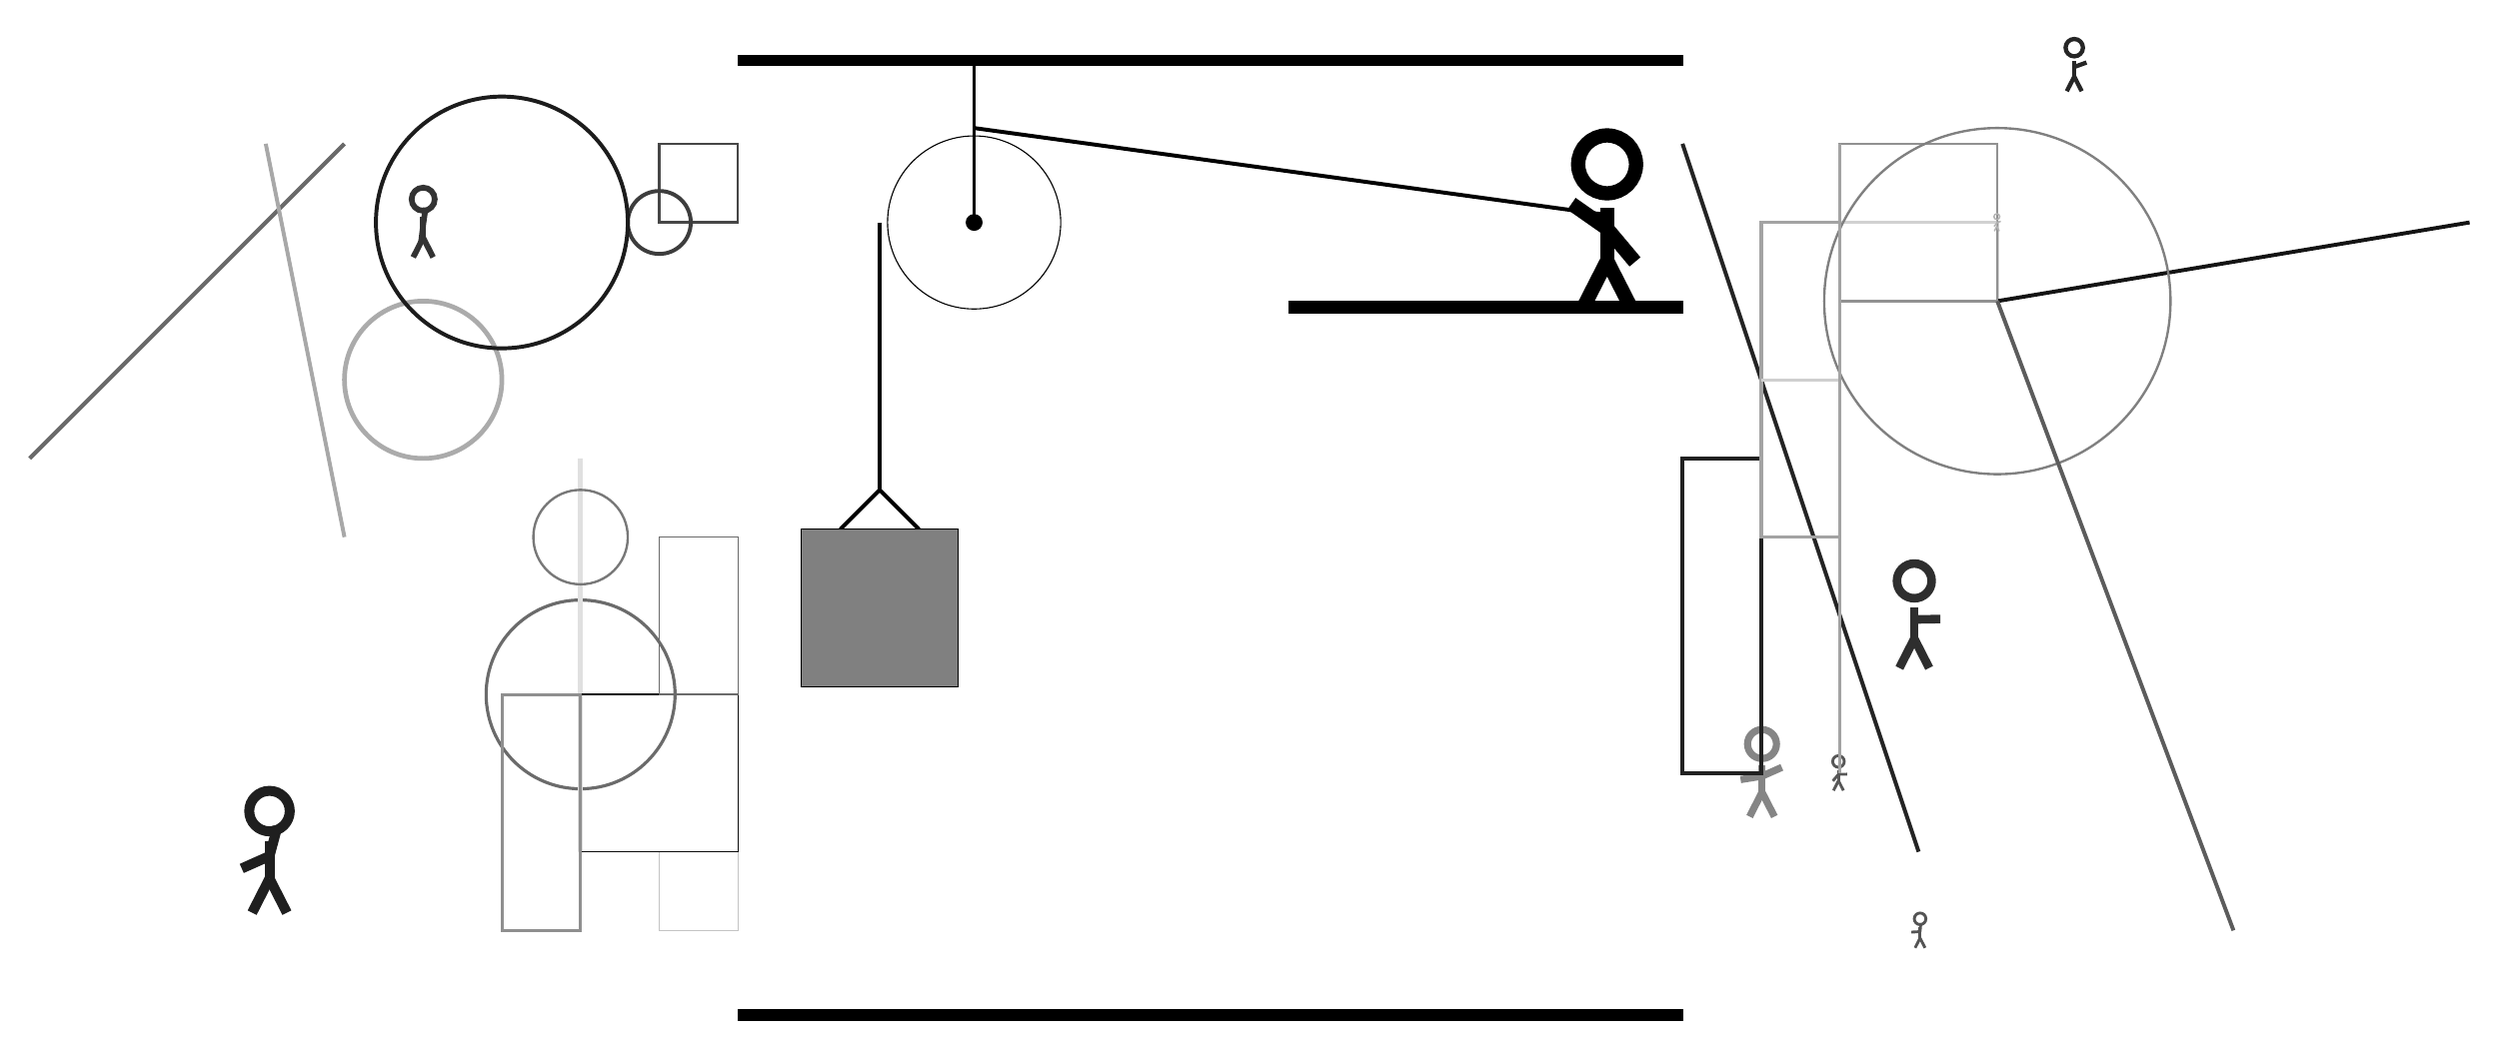
\begin{tikzpicture}
			%%%%% START %%%%%
			
			\draw[fill=black] (-2, 9) rectangle (10, 9.125);
			
			\draw (1, 7) circle (1.1);
			\draw[fill=black] (1, 7) circle (0.1);
			\draw[line width=0.5mm] (1, 9) -- (1, 7);
			
			\draw[line width=0.5mm](-0.7, 3.1) --  (-0.2, 3.6) -- (0.3, 3.1);
			\draw[fill=black!50] (-1.2, 3.1) rectangle (0.8, 1.1);
			
			\draw[line width=0.5mm](-0.2, 7) -- (-0.2, 3.6);
			\centerarc[line width=0.5mm](1, 7)(90:180:1.2000000000000002)
			\draw[line width=0.5mm](1, 8.2) -- (9, 7.1);
			
			\draw [line width=0.4mm, color=black!58](-4, 1) circle (1.2);
			
			\draw[line width=0.5mm, color=black!59](-7, 8) -- (-11, 4);
			\draw[line width=0.6mm, color=black!12] (-4, 4) rectangle (-4, -1);
			\node[line width=0.7mm, color=black!66] at (12, 0) {\Strichmaxerl[2][50][1]};
			\node[line width=0.6mm, color=black!88] at (-8, -1) {\Strichmaxerl[7][24][75]};
			\draw[line width=0.4mm, color=black!18] (12, 6) rectangle (14, 7);
			\node[line width=0.2mm, color=black!48] at (11, 0) {\Strichmaxerl[5][9][24]};
			
			\node[line width=0.6mm, color=black!80] at (-6, 7) {\Strichmaxerl[4][83][82]};
			\draw[line width=0.5mm, color=black!92](14, 6) -- (20, 7);
			\node[line width=0.7mm, color=black!85] at (15, 9) {\Strichmaxerl[3][90][20]};
			
			\draw[line width=0.2mm, color=black!23] (-3, -1) rectangle (-2, -2);
			
			\draw [line width=0.3mm, color=black!53](-4, 3) circle (0.6);
			\draw[line width=0.3mm, color=black!72] (-3, 7) rectangle (-2, 8);
			
			\draw[line width=0.3mm, color=black!43] (12, 8) rectangle (14, 6);
			\draw[line width=0.2mm, color=black!95] (-4, -1) rectangle (-2, 1);
			\draw[line width=0.5mm, color=black!87] (11, 4) rectangle (10, 0);
			\draw[line width=0.2mm, color=black!58] (-3, 3) rectangle (-2, 1);
			\draw[line width=0.5mm, color=black!86](10, 8) -- (13, -1);
			\draw [line width=0.5mm, color=black!76](-3, 7) circle (0.4);
			\draw [line width=0.3mm, color=black!50](14, 6) circle (2.2);
			\node[line width=0.6mm, color=black!82] at (13, 2) {\Strichmaxerl[6][90][1]};
			
			\draw[line width=0.4mm, color=black!36] (12, 3) rectangle (11, 7);
			\draw[line width=0.4mm, color=black!44] (-4, -2) rectangle (-5, 1);
			\node[line width=0.3mm, color=black!30] at (14, 7) {\Strichmaxerl[1][51][25]};
			\draw[line width=0.4mm, color=black!19] (11, 5) rectangle (12, 5);
			
			\draw[line width=0.5mm, color=black!34](-7, 3) -- (-8, 8);
			\draw[line width=0.5mm, color=black!64](14, 6) -- (17, -2);
			\draw[line width=0.4mm, color=black!36] (12, 8) rectangle (12, 0);
			
			\draw [line width=0.6mm, color=black!33](-6, 5) circle (1.0);
			
			\draw [line width=0.5mm, color=black!89](-5, 7) circle (1.6);
			\node[line width=0.7mm, color=black!67] at (13, -2) {\Strichmaxerl[2][3][85]};
			
			
			\node at (9, 7) {\Strichmaxerl[10][-35][-50]};
			\draw[fill=black] (5, 6) rectangle (10, 5.85);
			
			\draw[fill=black] (-2, -3) rectangle (10, -3.15);
			
			%%%%% END %%%%%
		\end{tikzpicture}
	\end{figure}	
\end{document}